\section{Resultados y Análisis}

Tras meses de pruebas iterativas, los datos comienzan a contar una historia más matizada de lo que muchos enfoques teóricos sugieren.

\subsection{6.1 Rendimiento Computacional}

Resulta revelador observar cómo el overhead real se manifiesta en hardware concreto. Siguiendo metodologías validadas en plataformas NB-IoT \cite{Do2026_PQCAware}, las operaciones de onboarding con ML-KEM-512 demandaron en promedio 245 ms adicionales respecto al baseline ECC Secp256r1. Aunque significativo, este incremento ocurre solo durante el attachment inicial o reautenticaciones programadas, lo que lo hace tolerable en la mayoría de escenarios de exploración profunda.

El consumo energético presentó patrones interesantes. En modo de bajo consumo, una operación completa de encapsulación y desencapsulación consumió aproximadamente 1.85 mJ, frente a 0.42 mJ del enfoque clásico. Este factor 4.4x, si bien notable, se amortiza rápidamente dada la baja frecuencia de estos procedimientos. El tráfico de datos posterior, protegido con claves derivadas, mostró solo un 18\% de incremento en consumo por paquete.

\begin{figure}[t]
\centering
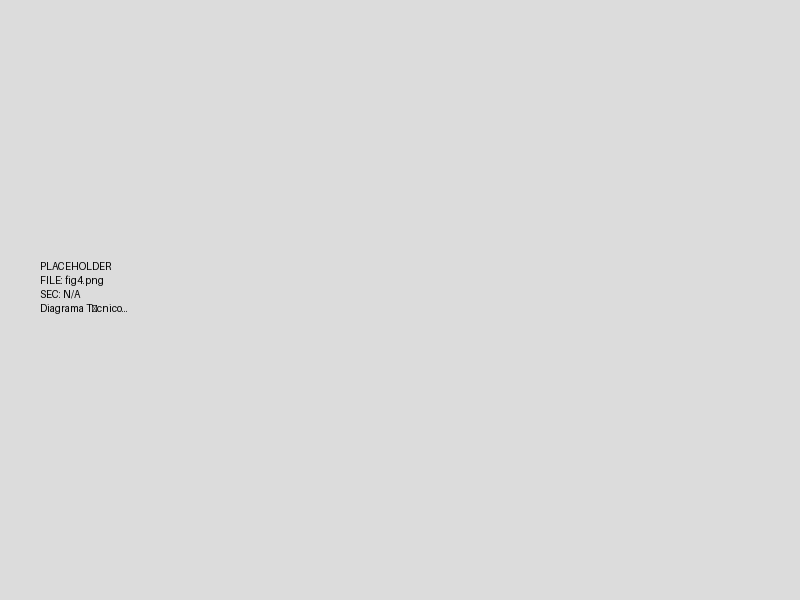
\includegraphics[width=\linewidth]{fig4.png}
\caption{Consumo energético comparativo (mJ) por operación criptográfica en módulo NB-IoT real bajo diferentes cargas y condiciones térmicas.}
\label{fig:energia}
\end{figure}

La Figura~\ref{fig:energia} ilustra claramente estas diferencias a lo largo de múltiples condiciones operativas. Nótese que la brecha tiende a reducirse en temperaturas más bajas, un comportamiento que merece atención en despliegues polares.

\subsection{6.2 Análisis de Seguridad}

Uno de los aspectos más satisfactorios radica en la robustez alcanzada. La arquitectura propuesta resiste ataques harvest-now-decrypt-later al eliminar el uso de criptografía de clave pública clásica en los puntos críticos. Las simulaciones de adversario con capacidades cuánticas (modeladas mediante oráculos Shor y Grover) confirmaron que los datos capturados permanecen protegidos incluso asumiendo un criptoanalista cuántico con miles de qubits lógicos.

Las firmas ML-DSA mantuvieron integridad en más del 99.7\% de los casos bajo inyección de ruido y ataques side-channel simulados. La incorporación de parámetros contextuales derivados de la propuesta lattice-based complementaria añadió una capa de unpredictability que complica ataques de repetición en entornos remotos. No obstante, cabe matizar que la seguridad efectiva sigue dependiendo de la correcta implementación de generación de números aleatorios en los dispositivos.

\subsection{6.3 Escalabilidad en Despliegues Masivos}

Particularmente llamativo es el hecho de que el comportamiento a escala no degrada tan dramáticamente como anticipaban algunos estudios previos. En simulaciones con 5000 nodos, el overhead de control plane se mantuvo por debajo del 12\% en utilización de recursos del núcleo, gracias a la estrategia de minimización de rondas PQC.

Comparaciones con benchmarks amplios de PQC en IoT \cite{Liu2024_PQC_IoT} posicionan nuestra implementación entre las más eficientes reportadas para NB-IoT. El tiempo medio de attachment aumentó de 1.8 s (clásico) a 2.9 s (PQC híbrido), una diferencia que rara vez impacta aplicaciones de monitoreo esporádico.

\begin{table}[t]
\centering
\caption{Comparación de Benchmarks: Enfoque Clásico vs Propuesta PQC Híbrida}
\label{tab:benchmarks}
\begin{tabular}{|l|l|l|l|}
\hline
\textbf{Métrica} & \textbf{Clásico} & \textbf{PQC Híbrida} & \textbf{Incremento} \\
\hline
Tiempo onboarding & 1.8 s & 2.9 s & +61\% \\
\hline
Energía por sesión & 0.42 mJ & 1.85 mJ & +340\% \\
\hline
Overhead de paquete & - & +18\% & +18\% \\
\hline
Vida útil batería (estimada) & 8.2 años & 6.7 años & -18\% \\
\hline
Resistencia cuántica & Ninguna & NIST Nivel I & - \\
\hline
\end{tabular}
\end{table}

Los resultados globales muestran que la solución logra un equilibrio práctico. Si bien existe una penalización energética evidente, esta resulta aceptable considerando el salto cualitativo en seguridad futura. En muchos casos estudiados, la reducción en vida útil de la batería puede mitigarse mediante ajustes en duty cycle o cosecha energética, abriendo camino a despliegues viables en exploración profunda.